\lecture{2}{22 Sep.}{}

\begin{recall}
    Erd\H{o}s's lower bound on \(R(k)\) colored the edges of \(K_n\) red and blue uniformly at random and applied the union bound over all \(k\)-sets of vertices: if
    \[
        \binom{n}{k} 2^{1 - \binom{k}{2}} < 1,
    \]
    then with positive probability no copy of \(K_k\) is monochromatic, so \(R(k) > n\).
\end{recall}

That argument never used that the colored objects are the edges of a complete graph. All it needed was a family of sets, the edge sets of the copies of \(K_k\), none of which may end up monochromatic. This lecture studies that coloring problem in its own right.

\section{Property B}\label{sec:property-B}

\subsection{Two-Colorability of Hypergraphs}

\begin{eg}[Chess Olympiad]\label{eg:chess-olympiad}
    A national team travels to the Chess Olympiad. Its members fill the following roles.
    \begin{center}
        \begin{minipage}[c]{0.4\linewidth}
            \begin{itemize}[topsep=0pt, itemsep=3pt, parsep=0pt]
                \item {\color{blue!70!black}\underline{\color{black}Team manager}}
                \item {\color{orange}\underline{\color{black}Team captains}}
                \item {\color{red!80!black}\underline{\color{black}Women}}
                \item \underline{Endgame specialists}
                \item Opening experts
                \item e4 players
                \item d4 players
                \item Sport psychologist
            \end{itemize}
        \end{minipage}%
        \hfill
        \begin{minipage}[c]{0.55\linewidth}
            \centering
            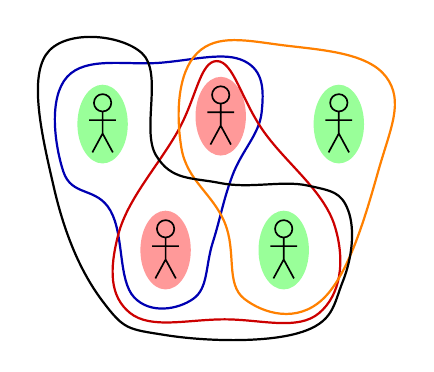
\begin{tikzpicture}[thick]
                % members, shaded by flight
                \foreach \x/\y/\flight in {0/1.6/green, 1.5/1.7/red, 3/1.6/green, 0.8/0/red, 2.3/0/green} {
                    \begin{scope}[shift={(\x,\y)}]
                        \fill[\flight!40] (0,0) ellipse (0.32 and 0.5);
                        \draw[semithick] (0,0.27) circle (0.11)
                            (0,0.16) -- (0,-0.12)
                            (-0.17,0.05) -- (0.17,0.05)
                            (0,-0.12) -- (-0.13,-0.36)
                            (0,-0.12) -- (0.13,-0.36);
                    \end{scope}
                }
                % roles: each curve encloses the members holding that role
                \draw[blue!70!black] plot[smooth cycle, tension=0.7] coordinates
                    {(-0.45,2.2) (0.75,2.38) (1.8,2.4) (2.02,1.75) (1.65,0.95) (1.4,0.1) (1.15,-0.62) (0.4,-0.6) (0.1,0.5) (-0.5,1.0)};
                \draw[red!80!black] plot[smooth cycle, tension=0.7] coordinates
                    {(1.45,2.4) (2.05,1.5) (2.95,0.3) (2.75,-0.8) (1.55,-0.88) (0.35,-0.8) (0.2,0.2) (0.95,1.5)};
                \draw[orange] plot[smooth cycle, tension=0.7] coordinates
                    {(1.2,2.5) (2.3,2.6) (3.6,2.2) (3.5,1.0) (2.8,-0.62) (1.8,-0.62) (1.55,0.35) (1.0,1.3)};
                \draw[black] plot[smooth cycle, tension=0.7] coordinates
                    {(-0.72,2.48) (0.5,2.5) (0.68,1.2) (1.5,0.85) (2.6,0.82) (3.12,0.5) (3.05,-0.4) (2.5,-1.05) (0.8,-1.08) (0.0,-0.65) (-0.62,0.8)};
            \end{tikzpicture}
        \end{minipage}
    \end{center}
    A member can hold several roles, e.g.\ a team captain who is also an endgame specialist, and a role is usually held by several members. The e4 and d4 players are those whose usual first move is 1.e4 and 1.d4, respectively. The team travels on two flights, and each flight should carry someone in every role, so that the team is complete even if the other flight is delayed.
\end{eg}

\begin{question}
    How can we assign the members to the \(2\) flights so that each flight has a person with every role?
\end{question}

The picture shows five members and the four underlined roles. Each closed curve encloses the members holding the role underlined in the same color, and the shading behind each member is a flight assignment: the members shaded red take one flight, those shaded green take the other. This answers the question, since each of the four curves contains both a red and a green member.

Abstractly, the data are a set of people with a family of subsets of it, one subset per role, and a flight assignment colors the people with two colors. This is the following structure.

\begin{definition}[Hypergraph]
    A \vocab{hypergraph} is a pair \(H = (V, E)\) of vertices \(V\) and edges \(E \subseteq 2^V\), where an edge is a subset of vertices. It is \vocab{\(k\)-uniform} if \(\abs{e} = k\) for all \(e \in E\).
\end{definition}

\begin{notation}
    \(2^V\) is the power set of \(V\), and \(V(H)\), \(E(H)\) are the vertex and edge sets of \(H\); all hypergraphs here are finite. For a set \(X\), \(\binom{X}{k}\) is the family of all \(k\)-element subsets of \(X\), and \([N] = \{1, \ldots, N\}\).
\end{notation}

\begin{remark}
    A graph is a \(2\)-uniform hypergraph: each of its edges is a set \(\{u, v\}\) of two vertices.
\end{remark}

\begin{definition}[Property B]
    A hypergraph has \vocab{Property B}, or is \vocab{two-colorable}, if we can two-color the vertices of it s.t.\ every edge has vertices of both \(2\) colors.
\end{definition}

Picture the two colors as the two halves of a box: put the red vertices in the left half and the blue vertices in the right half. Property B asks for a way to place every vertex so that each edge crosses the dividing line, i.e.\ has a vertex on both sides.
\begin{center}
    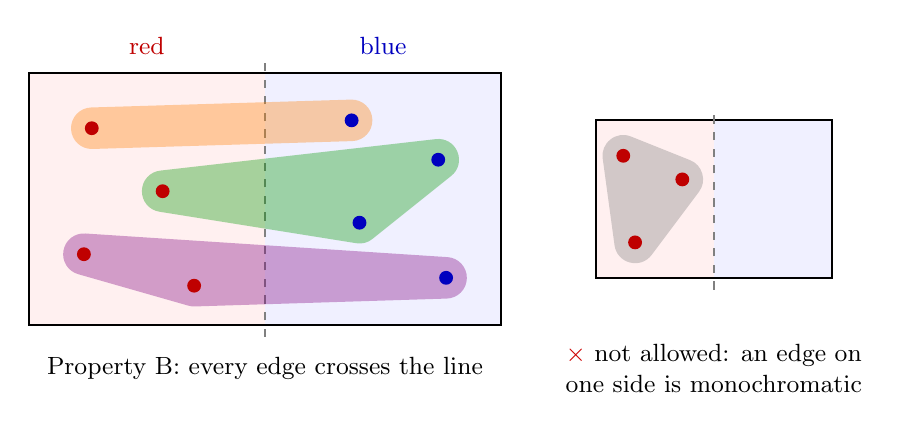
\begin{tikzpicture}[thick, every node/.style={font=\small}]
        % the box: left half = red, right half = blue
        \fill[red!6] (0,0) rectangle (3,3.2);
        \fill[blue!6] (3,0) rectangle (6,3.2);
        \draw (0,0) rectangle (6,3.2);
        \draw[dashed, gray] (3,-0.15) -- (3,3.35);
        \node[red!75!black] at (1.5,3.55) {red};
        \node[blue!75!black] at (4.5,3.55) {blue};
        \foreach \name/\x/\y in {l1/0.8/2.5, l2/1.7/1.7, l3/0.7/0.9, l4/2.1/0.5,
                                 r1/4.1/2.6, r2/5.2/2.1, r3/4.2/1.3, r4/5.3/0.6}
            \coordinate (\name) at (\x,\y);
        % edges, drawn as shaded hulls; each one crosses the dashed line
        \begin{scope}[transparency group, opacity=0.35]
            \draw[orange, line width=15pt, line cap=round] (l1) -- (r1);
        \end{scope}
        \begin{scope}[transparency group, opacity=0.35]
            \filldraw[green!60!black, line width=15pt, line join=round] (l2) -- (r2) -- (r3) -- cycle;
        \end{scope}
        \begin{scope}[transparency group, opacity=0.35]
            \filldraw[violet, line width=15pt, line join=round] (l3) -- (l4) -- (r4) -- cycle;
        \end{scope}
        \foreach \name in {l1,l2,l3,l4} \fill[red!75!black] (\name) circle (2.5pt);
        \foreach \name in {r1,r2,r3,r4} \fill[blue!75!black] (\name) circle (2.5pt);
        \node at (3,-0.55) {Property B: every edge crosses the line};

        % a forbidden edge for contrast
        \begin{scope}[xshift=7.2cm, yshift=0.6cm]
            \fill[red!6] (0,0) rectangle (1.5,2);
            \fill[blue!6] (1.5,0) rectangle (3,2);
            \draw (0,0) rectangle (3,2);
            \draw[dashed, gray] (1.5,-0.15) -- (1.5,2.15);
            \coordinate (b1) at (0.35,1.55);
            \coordinate (b2) at (1.1,1.25);
            \coordinate (b3) at (0.5,0.45);
            \begin{scope}[transparency group, opacity=0.35]
                \filldraw[gray, line width=15pt, line join=round] (b1) -- (b2) -- (b3) -- cycle;
            \end{scope}
            \foreach \name in {b1,b2,b3} \fill[red!75!black] (\name) circle (2.5pt);
            \node[align=center] at (1.5,-1.15) {{\color{red!80!black}\(\bm{\times}\)} not allowed: an edge on\\one side is monochromatic};
        \end{scope}
    \end{tikzpicture}
\end{center}
Equivalently, there is a coloring \(\chi \colon V \to \{\text{red}, \text{blue}\}\) under which no edge is \vocab{monochromatic}, i.e.\ has all of its vertices of one color. The name refers to Felix Bernstein, who studied this property in 1908.

In \autoref{eg:chess-olympiad}, the vertices are the members, each role is an edge, and a flight assignment is a two-coloring, so the question asks whether this hypergraph has Property B. The shading shows that the drawn part, a \(3\)-uniform hypergraph with five vertices and four edges, does.

\subsection{Connection to Ramsey Numbers}

The Ramsey problem is a question about Property B for one particular family of hypergraphs. Given \(n\) and \(k\), build the hypergraph \(H_{n,k}\) with
\[
    V(H_{n,k}) = E(K_n), \qquad E(H_{n,k}) = \{\, E(K) : K \text{ is a copy of } K_k \text{ in } K_n \,\}.
\]
Its vertices are the \(\binom{n}{2}\) edges of \(K_n\). It has one edge for each \(k\)-set \(S\) of vertices of \(K_n\), consisting of the \(\binom{k}{2}\) edges of \(K_n\) inside \(S\). Thus \(H_{n,k}\) is a \(\binom{k}{2}\)-uniform hypergraph with \(\binom{n}{k}\) edges.

\begin{eg}[\(n = 5\), \(k = 3\)]
    Write \(ij\) for the edge of \(K_5\) between the vertices \(i\) and \(j\).
    \begin{center}
        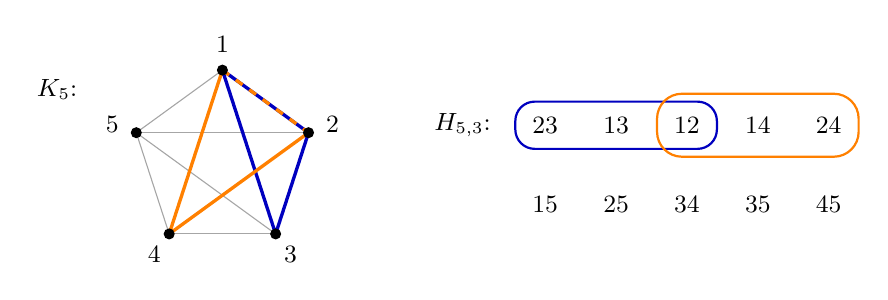
\begin{tikzpicture}[thick, every node/.style={font=\small}]
            \foreach \idx in {1,...,5} {
                \coordinate (k-\idx) at ({90-72*(\idx-1)}:1.15);
                \node at ({90-72*(\idx-1)}:1.47) {$\idx$};
            }
            \foreach \first/\second in {1/5, 2/5, 3/4, 3/5, 4/5}
                \draw[gray!70, thin] (k-\first) -- (k-\second);
            \draw[blue!75!black, very thick] (k-1) -- (k-3) (k-2) -- (k-3);
            \draw[orange, very thick] (k-1) -- (k-4) (k-2) -- (k-4);
            \draw[blue!75!black, very thick] (k-1) -- (k-2);
            \draw[orange, very thick, dash pattern=on 3pt off 3pt] (k-1) -- (k-2);
            \foreach \idx in {1,...,5} \fill (k-\idx) circle (2pt);
            \node at (-2.1,0.9) {$K_5$:};

            \begin{scope}[xshift=4.1cm, yshift=0.45cm]
                \node at (-1.05,0) {$H_{5,3}$:};
                \foreach \pair [count=\idx from 0] in {23, 13, 12, 14, 24}
                    \node at (0.9*\idx,0) {$\pair$};
                \foreach \pair [count=\idx from 0] in {15, 25, 34, 35, 45}
                    \node at (0.9*\idx,-1) {$\pair$};
                \draw[blue!75!black, rounded corners=7pt] (-0.38,-0.3) rectangle (2.18,0.3);
                \draw[orange, rounded corners=9pt] (1.42,-0.4) rectangle (3.98,0.4);
            \end{scope}
        \end{tikzpicture}
    \end{center}
    The ten vertices of \(H_{5,3}\) are the ten edges of \(K_5\), and its ten edges are the triangles of \(K_5\), each a set of three edges of \(K_5\). Only two triangles are drawn. The blue triangle \(123\) is the edge \(\{12, 13, 23\}\) of \(H_{5,3}\), and the orange triangle \(124\) is the edge \(\{12, 14, 24\}\). These two edges of \(H_{5,3}\) share the vertex \(12\) because the two triangles share the edge \(12\), drawn in both colors. The colors only mark the two triangles; they are not an edge-coloring.
\end{eg}

A red/blue coloring of the edges of \(K_n\) is the same thing as a two-coloring of the vertices of \(H_{n,k}\), and a copy of \(K_k\) is monochromatic exactly when the corresponding edge of \(H_{n,k}\) is. Hence \(K_n\) has a coloring without a monochromatic \(K_k\) iff \(H_{n,k}\) has Property B, and
\[
    R(k) = \min \{\, n : H_{n,k} \text{ does not have Property B} \,\}.
\]
Unfolding the definition of Property B, \(H_{n,k}\) is without Property B iff every two-coloring of its vertices leaves some edge monochromatic, so
\[
    R(k) = \min \left\{ n : \forall \chi \colon V(H_{n,k}) \to \{\text{red}, \text{blue}\},\ \exists\, e \in E(H_{n,k}) \text{ monochromatic under } \chi \right\}.
\]
Since \(V(H_{n,k}) = E(K_n)\), such a \(\chi\) is a red/blue coloring of the edges of \(K_n\), and a monochromatic \(e \in E(H_{n,k})\) is a monochromatic copy of \(K_k\); this is word for word the definition of \(R(k)\) from Lecture 1.

\begin{remark}\label{rmk:property-B-bipartite}
    For \(k = 2\), Property B \(\equiv\) bipartite. Here \(k\) is the uniformity, not the \(k\) of \(R(k)\): a \(2\)-uniform hypergraph is a graph, and an edge \(\{u, v\}\) sees both colors iff \(u\) and \(v\) get different colors. So a two-coloring without monochromatic edges is exactly a partition of \(V\) into two independent sets, i.e.\ a bipartition. Property B thus generalizes bipartiteness to hypergraphs; for instance, \(C_5\) from Lecture 1, and every other odd cycle, does not have Property B.
\end{remark}

\subsection{The Extremal Problem}

Every edge is one more constraint on the coloring, so a hypergraph with few edges should be two-colorable. We measure the size of a hypergraph by its number of edges and leave the number of vertices unrestricted.

\begin{question}[Extremal problem]
    How small can a \(k\)-uniform hypergraph be if it does not have Property B?
\end{question}

\begin{definition}
    \[
        m(k) \coloneqq \min \{\, m : \exists\, k\text{-uniform hypergraph } H = (V, E),\ \abs{E} = m,\ \text{without Property B} \,\}.
    \]
    Unfolding the definition of Property B, \(H\) is without Property B iff every two-coloring of \(V\) leaves some edge monochromatic, so
    \[
        m(k) = \min \left\{ m :
        \begin{array}{l}
            \exists\, H = (V, E) \text{ with } \abs{E} = m \text{ and } \abs{e} = k \ \forall e \in E, \text{ s.t.} \\
            \forall \chi \colon V \to \{\text{red}, \text{blue}\},\ \exists\, e \in E \text{ monochromatic under } \chi
        \end{array}
        \right\}.
    \]
\end{definition}

This minimum exists only if the set on the right is nonempty, i.e.\ if some \(k\)-uniform hypergraph fails to have Property B. That is indeed the case: the hypergraph \(\bigl([2k-1], \binom{[2k-1]}{k}\bigr)\) in \autoref{prop:m-upper} has no Property B, so \(\binom{2k-1}{k}\) belongs to the set and \(m(k)\) is well defined. By minimality, every \(k\)-uniform hypergraph with fewer than \(m(k)\) edges has Property B, while some \(k\)-uniform hypergraph with \(m(k)\) edges does not. As with every extremal problem, determining \(m(k)\) has two halves, but since \(m(k)\) is a minimum their roles are swapped: a construction without Property B gives an upper bound, and a proof that every small hypergraph has Property B gives a lower bound.

\begin{proposition}[Erd\H{o}s, 1963]\label{prop:m-lower}
    \[
        m(k) \ge 2^{k-1}.
    \]
\end{proposition}

\begin{proof}
    WTS: If \(H = (V, E)\) is a \(k\)-uniform hypergraph with \(m < 2^{k-1}\) edges, then it is two-colorable.

    Color the vertices red and blue independently and uniformly. Let \(E = \{e_1, e_2, \ldots, e_m\}\), and let \(A_i\) be the event that the edge \(e_i\) is monochromatic. The edge \(e_i\) has exactly \(k\) vertices with independent colors, and it is monochromatic iff they are all red or all blue, so
    \[
        \mathbb{P}(A_i) = 2 \left( \frac{1}{2} \right)^k = \left( \frac{1}{2} \right)^{k-1}.
    \]
    The events \(A_i\) need not be independent, since edges may share vertices, but the union bound does not need independence:
    \[
        \mathbb{P}(\exists \text{ monochromatic edge}) = \mathbb{P}\left( \bigcup_{i=1}^{m} A_i \right) \le \sum_{i=1}^{m} \mathbb{P}(A_i) = m \cdot 2^{-(k-1)} < 1 \quad \text{for } m < 2^{k-1}.
    \]
    Taking complements, and using that an event of positive probability contains at least one outcome,
    \begin{gather*}
        \mathbb{P}(\nexists \text{ monochromatic edge}) > 0 \\
        \Downarrow \\
        \exists \text{ a two-coloring of vertices where every edge sees both colors} \\
        \Downarrow \\
        H \text{ is two-colorable.} \qedhere
    \end{gather*}
\end{proof}

\begin{remark}
    Applied to \(H_{n,k}\), which is \(\binom{k}{2}\)-uniform with \(\binom{n}{k}\) edges, \autoref{prop:m-lower} says: if \(\binom{n}{k} < 2^{\binom{k}{2} - 1}\), then \(H_{n,k}\) has Property B, i.e.\ \(R(k) > n\). This is exactly the condition \(\binom{n}{k} 2^{1 - \binom{k}{2}} < 1\) in Erd\H{o}s's lower bound on \(R(k)\), and the proof above is the same computation with \(K_n\) replaced by an arbitrary hypergraph.
\end{remark}

\subsection{Upper Bounds on \texorpdfstring{\(m(k)\)}{m(k)}}

An upper bound on \(m(k)\) comes from exhibiting one \(k\)-uniform hypergraph without Property B that has few edges.

\begin{proposition}\label{prop:m-upper}
    \(m(1) = 1\), \(m(2) = 3\), and for every \(k \ge 1\),
    \[
        m(k) \le \binom{2k-1}{k} \sim c \, \frac{2^{2k}}{\sqrt{k}}, \qquad c = \frac{1}{2\sqrt{\pi}}.
    \]
\end{proposition}

\begin{center}
    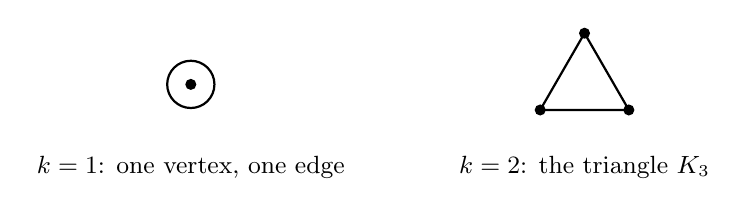
\begin{tikzpicture}[thick, every node/.style={font=\small}]
        \fill (0,0) circle (2pt);
        \draw (0,0) circle (0.3);
        \node at (0,-1.05) {$k = 1$: one vertex, one edge};
        \begin{scope}[xshift=5cm]
            \foreach \idx/\angle in {1/90, 2/210, 3/330}
                \coordinate (t-\idx) at (\angle:0.65);
            \draw (t-1) -- (t-2) -- (t-3) -- cycle;
            \foreach \idx in {1,2,3} \fill (t-\idx) circle (2pt);
            \node at (0,-1.05) {$k = 2$: the triangle $K_3$};
        \end{scope}
    \end{tikzpicture}
\end{center}

\begin{proof}
    \hfill
    \begin{enumerate}[(1), beginpenalty=10000]
        \item \(m(1) = 1\): Take one vertex \(v\) and the single edge \(\{v\}\) (left picture above). This edge has only one vertex, so it is monochromatic under every coloring. A hypergraph with no edges has Property B vacuously, so \(m(1) = 1\). In \autoref{eg:chess-olympiad}, an edge of size \(1\) is a role held by a single member, e.g.\ a lone sport psychologist: then no flight assignment works.

        \item \(m(2) = 3\): A \(2\)-uniform hypergraph is a graph, and by \autoref{rmk:property-B-bipartite} it is without Property B iff it is not bipartite. So \(m(2)\) is the fewest edges of a non-bipartite graph, and we show two things.
        \begin{itemize}
            \item \(m(2) \le 3\): The triangle \(K_3\) (right picture above) is without Property B. Take any two-coloring of its three vertices. By the pigeonhole principle, two of the three vertices get the same color, and since every two vertices of \(K_3\) are adjacent, the edge between them is monochromatic.
            \item \(m(2) \ge 3\): Every graph \(G\) with at most two edges has Property B. We color the vertices of the edges red and blue as below, and all other vertices, which lie in no edge, arbitrarily.
            \begin{center}
                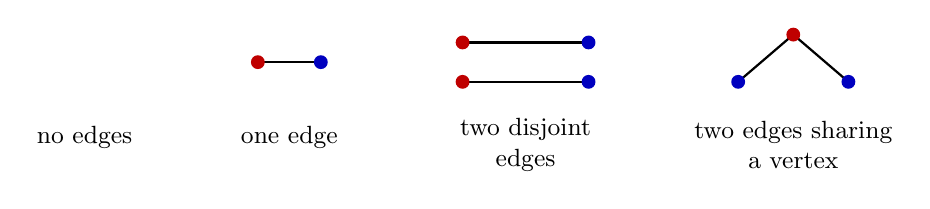
\begin{tikzpicture}[thick, every node/.style={font=\small}]
                    \node at (0,-0.75) {no edges};
                    \node at (0,0.2) {$\varnothing$};
                    \begin{scope}[xshift=2.6cm]
                        \draw (-0.4,0.2) -- (0.4,0.2);
                        \fill[red!75!black] (-0.4,0.2) circle (2.5pt);
                        \fill[blue!75!black] (0.4,0.2) circle (2.5pt);
                        \node at (0,-0.75) {one edge};
                    \end{scope}
                    \begin{scope}[xshift=5.6cm]
                        \draw (-0.8,0.45) -- (0.8,0.45) (-0.8,-0.05) -- (0.8,-0.05);
                        \foreach \y in {0.45,-0.05} {
                            \fill[red!75!black] (-0.8,\y) circle (2.5pt);
                            \fill[blue!75!black] (0.8,\y) circle (2.5pt);
                        }
                        \node[align=center] at (0,-0.85) {two disjoint\\edges};
                    \end{scope}
                    \begin{scope}[xshift=9cm]
                        \draw (-0.7,-0.05) -- (0,0.55) -- (0.7,-0.05);
                        \fill[red!75!black] (0,0.55) circle (2.5pt);
                        \fill[blue!75!black] (-0.7,-0.05) circle (2.5pt);
                        \fill[blue!75!black] (0.7,-0.05) circle (2.5pt);
                        \node[align=center] at (0,-0.85) {two edges sharing\\a vertex};
                    \end{scope}
                \end{tikzpicture}
            \end{center}
            With one edge \(\{u, v\}\), color \(u\) red and \(v\) blue. With two disjoint edges \(\{a, b\}\), \(\{c, d\}\), color \(a, c\) red and \(b, d\) blue. With two edges \(\{a, b\}\), \(\{a, c\}\) sharing the vertex \(a\), color \(a\) red and \(b, c\) blue. In every case each edge has one red and one blue endpoint, so no edge is monochromatic.
        \end{itemize}
        Hence \(m(2) = 3\). Note that \autoref{prop:m-lower} alone only gives \(m(2) \ge 2^{2-1} = 2\), so the case check above is needed for the lower bound.

        \item \(m(k) \le \binom{2k-1}{k}\): Consider \(2k - 1\) vertices and let any \(k\) of them form an edge, i.e.\ take the hypergraph \(\left( [2k-1], \binom{[2k-1]}{k} \right)\). In a two-coloring of \(2k - 1\) vertices, by the pigeonhole principle, some color is used on at least \(k\) vertices, and any \(k\) of these form a monochromatic edge.
        \begin{center}
            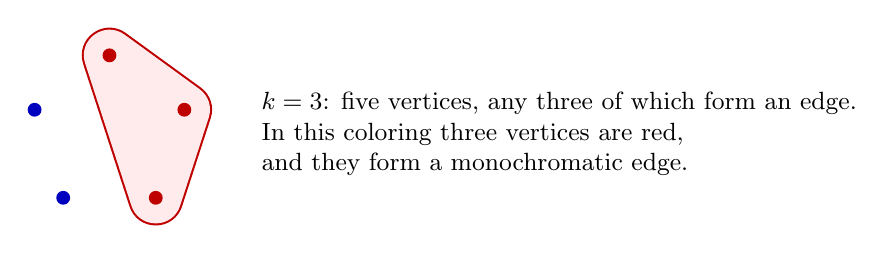
\begin{tikzpicture}[thick, every node/.style={font=\small}]
                \foreach \idx in {1,...,5}
                    \coordinate (p-\idx) at ({90-72*(\idx-1)}:1);
                % the edge {1,2,3}: its convex hull, widened by a thick round-joined stroke
                \draw[red!75!black, line width=20pt, line join=round] (p-1) -- (p-2) -- (p-3) -- cycle;
                \filldraw[red!8, line width=18.5pt, line join=round] (p-1) -- (p-2) -- (p-3) -- cycle;
                \foreach \idx/\col in {1/red, 2/red, 3/red, 4/blue, 5/blue}
                    \fill[\col!75!black] (p-\idx) circle (2.5pt);
                \node[align=left, anchor=west] at (1.8,0)
                    {$k = 3$: five vertices, any three of which form an edge.\\In this coloring three vertices are red,\\and they form a monochromatic edge.};
            \end{tikzpicture}
        \end{center}
        So this hypergraph does not have Property B, and \(m(k) \le \binom{2k-1}{k}\). For \(k = 1, 2\), it is exactly the edge \(\{v\}\) and the triangle above, so the bound is tight there.

        \item Asymptotics: By Pascal's rule and \(\binom{2k-1}{k-1} = \binom{2k-1}{k}\),
        \[
            \binom{2k}{k} = \binom{2k-1}{k-1} + \binom{2k-1}{k} = 2 \binom{2k-1}{k},
        \]
        and Stirling's formula \(N! \sim \sqrt{2\pi N} (N/e)^N\) gives
        \[
            \binom{2k}{k} = \frac{(2k)!}{(k!)^2} \sim \frac{\sqrt{4\pi k}\, (2k/e)^{2k}}{2\pi k\, (k/e)^{2k}} = \frac{4^k}{\sqrt{\pi k}}.
        \]
        Hence \(\binom{2k-1}{k} = \frac{1}{2} \binom{2k}{k} \sim \frac{1}{2\sqrt{\pi}} \cdot \frac{2^{2k}}{\sqrt{k}}\).\qedhere
    \end{enumerate}
\end{proof}

\begin{remark}
    Together, \autoref{prop:m-lower} and \autoref{prop:m-upper} give
    \[
        2^{k-1} \le m(k) \le (1 + o(1)) \frac{4^k}{2\sqrt{\pi k}}.
    \]
    Both bounds are exponential in \(k\), with bases \(2\) and \(4\), the same kind of gap as \(\sqrt{2}^{\,k} \lesssim R(k) \le 4^k\) for Ramsey numbers. Unlike for Ramsey numbers, this gap can be closed up to a polynomial factor: the base \(2\) of the lower bound is the right one. The explicit hypergraph \(\bigl([2k-1], \binom{[2k-1]}{k}\bigr)\) is wasteful because it uses every \(k\)-set of its vertices, and the next subsection shows that a \emph{random} choice of far fewer \(k\)-sets on a larger vertex set already fails to have Property B.
\end{remark}

\subsection{A Random Construction}

To show that \(m(k) \le m\) we must exhibit a \(k\)-uniform hypergraph with \(m\) edges and without Property B. Instead of constructing one, we pick one at random and show that it fails to have Property B with positive probability.

\begin{theorem}[Erd\H{o}s, 1964]\label{thm:m-upper-random}
    \(m(k) = O(k^2 2^k)\), i.e.\ there is a constant \(C > 0\) s.t.\ \(m(k) \le C k^2 2^k\) for all large enough \(k\).
\end{theorem}

\begin{proof}
    Idea: take a random hypergraph \(H\).
    \begin{itemize}
        \item Fix a set \(V\) of \(n\) vertices.
        \item Choose \(m\) edges \(e_1, e_2, \ldots, e_m\) uniformly at random from \(\binom{V}{k}\), independently of each other.
    \end{itemize}
    The numbers \(n\) and \(m\) will be chosen later. The same \(k\)-set may be picked twice; then \(H\) has fewer than \(m\) distinct edges, and deleting repeated copies of an edge does not affect Property B. So it suffices to show
    \[
        \mathbb{P}(H \text{ is not two-colorable}) > 0 \implies m(k) \le \abs{E(H)} \le m.
    \]
    Now the random object is the hypergraph, and the bad event is that \(H\) \emph{is} two-colorable, i.e.\ for some two-coloring \(\chi \colon V \to \{\text{red}, \text{blue}\}\) there is no monochromatic edge. There are \(2^n\) colorings, so we fix one, bound the probability that it works, and take a union bound over all of them. This is the reverse of \autoref{prop:m-lower}, where the hypergraph was fixed and the coloring was random.

    Let \(\chi\) be a two-coloring of \(V\), and let \(A_\chi\) be the event that none of \(e_1, e_2, \ldots, e_m\) is monochromatic under \(\chi\). Consider one edge \(e_i\). Since \(e_i\) is uniformly random,
    \[
        \mathbb{P}(e_i \text{ is monochromatic under } \chi) = \frac{\#\text{ monochromatic } k\text{-sets}}{\#\text{ possible } k\text{-sets}} = \frac{\binom{r}{k} + \binom{n-r}{k}}{\binom{n}{k}},
    \]
    where \(r\) is the number of red vertices under \(\chi\). The function \(x \mapsto \binom{x}{k} = \frac{x(x-1) \cdots (x-k+1)}{k!}\), extended by \(0\) for \(x < k - 1\), is convex on \([0, \infty)\).\footnote{On \([k-1, \infty)\) it is a polynomial all of whose roots are \(\le k - 1\), so by Rolle's theorem all of its derivatives are positive there; gluing it to the constant \(0\) at \(x = k - 1\), where both vanish and the right derivative is \(\ge 0\), keeps it convex.} By convexity,
    \[
        \frac{1}{2} \left[ \binom{r}{k} + \binom{n-r}{k} \right] \ge \binom{\frac{1}{2}(r + n - r)}{k} \implies \binom{r}{k} + \binom{n-r}{k} \ge 2 \binom{n/2}{k},
    \]
    that is, a balanced coloring has the fewest monochromatic \(k\)-sets. Hence, for every \(\chi\),
    \[
        \mathbb{P}(e_i \text{ is monochromatic under } \chi) \ge \frac{2 \binom{n/2}{k}}{\binom{n}{k}} \eqqcolon p,
    \]
    where \(\binom{n/2}{k}\) is the polynomial above evaluated at \(x = n/2\), so \(n\) need not be even. The edges are chosen independently, so
    \begin{align*}
        \mathbb{P}(A_\chi) = \mathbb{P}(\nexists \text{ monochromatic edge under } \chi)
        &= \prod_{i=1}^{m} \bigl( 1 - \mathbb{P}(e_i \text{ is monochromatic under } \chi) \bigr) \\
        &\le (1 - p)^m,
    \end{align*}
    and by the union bound over the \(2^n\) colorings,
    \[
        \mathbb{P}(H \text{ is two-colorable}) = \mathbb{P}\Bigl( \bigcup_{\chi} A_\chi \Bigr) \le \sum_{\chi} \mathbb{P}(A_\chi) \le 2^n (1 - p)^m.
    \]
    We must choose \(n\) and \(m\) so that \(2^n (1 - p)^m < 1\), where \(p = 2\binom{n/2}{k} / \binom{n}{k}\). Using \(1 - x < e^{-x}\) for \(x > 0\),
    \[
        2^n (1 - p)^m < 2^n e^{-pm} = e^{n \ln 2 - pm}, \qquad \text{where } e^{n \ln 2 - pm} \le 1 \iff m \ge \frac{n \ln 2}{p}.
    \]
    We will take \(m = \bigl\lfloor \frac{n \ln 2}{p} \bigr\rfloor + 1\), and choose \(n\) to minimize it. For this we need \(p\) precisely as a function of \(n\) and \(k\). Writing out both binomial coefficients, the \(i = 0\) factor equals \(\frac{1}{2}\) and cancels the \(2\):
    \begin{align*}
        p = \frac{2 \binom{n/2}{k}}{\binom{n}{k}}
        &= 2 \prod_{i=0}^{k-1} \frac{\frac{n}{2} - i}{n - i}
        = \prod_{i=1}^{k-1} \frac{n - 2i}{2(n - i)}
        = \prod_{i=1}^{k-1} \left( \frac{1}{2} - \frac{i}{2(n-i)} \right)
        = \frac{1}{2^{k-1}} \prod_{i=1}^{k-1} \left( 1 - \frac{i}{n - i} \right) \\
        &= \frac{1}{2^{k-1}} \prod_{i=1}^{k-1} \left( 1 - \frac{i}{n} + O\Bigl( \frac{i^2}{n^2} \Bigr) \right)
        = \frac{1}{2^{k-1}} \prod_{i=1}^{k-1} e^{-\frac{i}{n} + O\left( \frac{i^2}{n^2} \right)} \\
        &= \frac{1}{2^{k-1}} \, e^{-\sum_{i=1}^{k-1} \left( \frac{i}{n} + O\left( \frac{i^2}{n^2} \right) \right)}
        = \frac{1}{2^{k-1}} \, e^{-\frac{k(k-1)}{2n} + O\left( \frac{k^3}{n^2} \right)}.
    \end{align*}
    Here we assumed \(n \ge 2k\), so that \(\frac{i}{n-i} \le 1\) and \(\frac{i}{n-i} = \frac{i}{n} + O(\frac{i^2}{n^2})\), and used \(1 - x = e^{-x + O(x^2)}\) for small \(x \ge 0\). Now, since
    \[
        m \approx \frac{n \ln 2}{p} = 2^{k-1} \, n \, e^{\frac{k(k-1)}{2n} + O\left( \frac{k^3}{n^2} \right)} \ln 2,
    \]
    we minimize \(n e^{k^2/(2n)}\) over \(n\): its derivative in \(n\) is \(e^{k^2/(2n)} (1 - \frac{k^2}{2n})\), which vanishes at \(n = \frac{k^2}{2}\). The optimal choice is thus \(n = c k^2\) with \(c = \frac{1}{2}\), rounded to an integer. Then \(\frac{k(k-1)}{2n} = 1 + O(\frac{1}{k})\) and \(\frac{k^3}{n^2} = O(\frac{1}{k})\), so
    \[
        m(k) \le m \le 2^{k-1} \cdot \frac{k^2}{2} \cdot e^{1 + O(1/k)} \ln 2 + 1 = (1 + o(1)) \, \frac{e \ln 2}{4} \, k^2 2^k \le C k^2 2^k. \qedhere
    \]
\end{proof}

\begin{remark}[Estimating binomial coefficients]
    Exact computation of \(p\) is not needed for \(O(k^2 2^k)\), only for the constant. The standard estimates
    \begin{gather*}
        \frac{(n-k)^k}{k!} \le \binom{n}{k} = \frac{n(n-1)(n-2) \cdots (n-k+1)}{k!} \le \frac{n^k}{k!}, \\
        \left( \frac{n}{k} \right)^k \le \binom{n}{k} = \frac{n(n-1) \cdots (n-k+1)}{k(k-1) \cdots (k-k+1)} \le \left( \frac{ne}{k} \right)^k
    \end{gather*}
    follow from bounding each factor \(n - i\) between \(n - k\) and \(n\), from \(\frac{n-i}{k-i} \ge \frac{n}{k}\), and from \(k! \ge (k/e)^k\). The first one already gives
    \[
        p = \frac{2 \binom{n/2}{k}}{\binom{n}{k}} \ge 2 \cdot \frac{(n/2 - k)^k / k!}{n^k / k!} = \frac{1}{2^{k-1}} \left( 1 - \frac{2k}{n} \right)^k \ge \frac{1}{2^{k-1}} e^{-4k^2/n} \quad \text{for } n \ge 4k,
    \]
    using \(1 - x \ge e^{-2x}\) for \(0 \le x \le \frac{1}{2}\). With \(n = 4k^2\) this yields \(m(k) \le (1 + o(1)) \, 2e \ln 2 \cdot k^2 2^k\), the same order with a worse constant.
\end{remark}

\subsection{Better Lower Bounds: Random Greedy Coloring}

Combining \autoref{prop:m-lower} and \autoref{thm:m-upper-random},
\begin{theorem}[Erd\H{o}s, 1963--64]
    \(2^{k-1} \le m(k) \le C k^2 2^k\) for some constant \(C > 0\).
\end{theorem}
Since then the lower bound has been improved by polynomial factors in \(k\), while the upper bound \(O(k^2 2^k)\) is still the best known.
\begin{theorem}[Radhakrishnan--Srinivasan, 2000]
    \(m(k) \ge c \sqrt{\frac{k}{\ln k}} \, 2^k\) for some constant \(c > 0\).
\end{theorem}
\begin{theorem}[Pluh\'ar, 2009]\label{thm:pluhar}
    \(m(k) \ge c \, k^{1/4} 2^k\) for some constant \(c > 0\).
\end{theorem}

We now prove \autoref{thm:pluhar}. The proof has two ideas: first a deterministic greedy coloring, whose failures we can describe exactly, and then a random order of the vertices, which makes such failures unlikely.

\begin{proof}
    The proof of \autoref{prop:m-lower} colored every vertex independently at random, which ignores the structure of \(H\) entirely. Instead:

    \textbf{Idea 1:} Color the vertices greedily. Order the vertices \(v_1, v_2, \ldots, v_n\), and consider the vertices one by one. Color \(v_i\) red, unless that creates a monochromatic (red) edge, i.e.\ unless some edge contains \(v_i\) and all of its other vertices are already colored red, in which case we color \(v_i\) blue. Colors are never changed afterwards.

    \begin{observation}
        \hfill
        \begin{enumerate}[(1)]
        \item No monochromatic red edge: when the last vertex of an edge is reached and all the others are red, it is colored blue.
        \item Monochromatic blue edges can occur. However, a vertex \(v\) is colored blue only because coloring it red would have completed a red edge. So every blue vertex \(v\) lies in some edge \(e\) such that all vertices of \(e\) other than \(v\) are red and come before \(v\) in the order.
        \end{enumerate}
    \end{observation}
    For example, in the \(4\)-uniform hypergraph below, order the twelve lower vertices first and the four top vertices last. The lower vertices are all colored red, since each vertical edge still has an uncolored top vertex. Each top vertex is then the last vertex of a vertical edge whose other vertices are red, so it is colored blue, and the horizontal edge ends up monochromatic blue.
    \begin{center}
        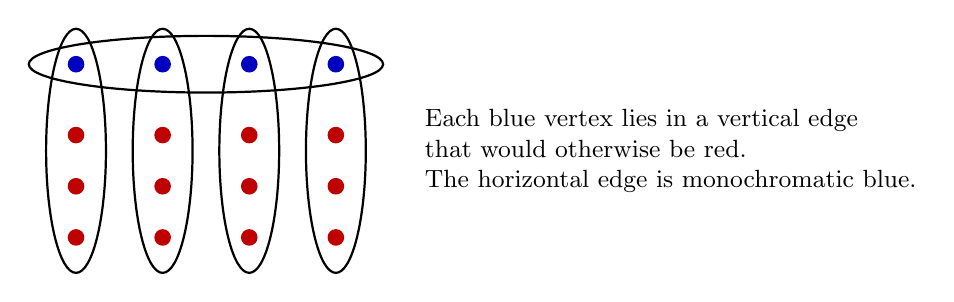
\begin{tikzpicture}[thick]
            \foreach \x in {0,1,2,3} {
                \draw (1.1*\x,0.35) ellipse (0.38 and 1.55);
                \fill[blue!75!black] (1.1*\x,1.45) circle (3pt);
                \foreach \y in {0.55,-0.1,-0.75}
                    \fill[red!75!black] (1.1*\x,\y) circle (3pt);
            }
            \draw (1.65,1.45) ellipse (2.25 and 0.36);
            \node[anchor=west, align=left, font=\small] at (4.3,0.35)
                {Each blue vertex lies in a vertical edge\\that would otherwise be red.\\The horizontal edge is monochromatic blue.};
        \end{tikzpicture}
    \end{center}
    We say the greedy coloring \emph{fails} if the coloring it produces is not a proper two-coloring, i.e.\ some edge is monochromatic. By (1), this happens exactly when some edge is monochromatic blue, as in the example. What must \(H\) and the order look like for this to happen? Suppose \(f\) is a monochromatic blue edge, and let \(v\) be the \emph{first} vertex of \(f\) in the order. By (2), \(v\) lies in an edge \(e\) whose other vertices are red and come before \(v\). Since all of \(f\) is blue, \(e \cap f = \{v\}\); and since \(v\) is the last vertex of \(e\) and the first vertex of \(f\), all of \(e\) comes before all of \(f\):
    \begin{center}
        \begin{tikzpicture}[thick]
            \draw (0,0) ellipse (1.35 and 0.42);
            \draw (2.3,0) ellipse (1.35 and 0.42);
            \foreach \x in {-0.9,-0.5} \fill[red!75!black] (\x,0) circle (2.5pt);
            \node at (-0.05,0) {$\cdots$};
            \fill[blue!75!black] (1.15,0) circle (2.5pt);
            \node[above, font=\small] at (1.15,0.42) {$v$};
            \node at (2.35,0) {$\cdots$};
            \foreach \x in {1.6,1.95,2.8,3.2} \fill[blue!75!black] (\x,0) circle (2.5pt);
            \node at (-0.3,-0.75) {$e$};
            \node at (2.6,-0.75) {$f$};
            \draw[-{Stealth}] (-1.4,-1.15) -- (3.7,-1.15) node[right, font=\small] {order};
        \end{tikzpicture}
    \end{center}
    We record what this argument shows. Note that it works for every order of the vertices.

    \begin{claim}\label{claim:greedy-fail}
        For any order of the vertices, if the greedy coloring produces a monochromatic edge, then there are edges \(e, f \in E(H)\) with \(\abs{e \cap f} = 1\) such that all of \(e\) comes before all of \(f\) in the order.
    \end{claim}

    Here \(e = f\) is possible only if \(f = \{v\}\) is an edge of size \(1\): then \(e = f = \{v\}\) and \(\abs{e \cap f} = 1\). Contrapositively, if no two edges meet in exactly one vertex, the greedy coloring cannot fail, whatever the order:

    \begin{corollary}
        If \(H\) is a hypergraph with \(\abs{e \cap f} \ne 1\) for all \(e, f \in E(H)\), then \(H\) is two-colorable.
    \end{corollary}

    \begin{subproof}
        Fix any order \(v_1, \ldots, v_n\) of the vertices and run the greedy coloring. It colors every vertex red or blue, so it gives a two-coloring \(\chi\) of \(V\); we show that no edge is monochromatic under \(\chi\).
        \begin{itemize}
            \item No edge is monochromatic red, by (1) of the observrvation.
            \item Suppose some edge \(f\) is monochromatic blue. By \autoref{claim:greedy-fail} there would be edges \(e, f\) with \(\abs{e \cap f} = 1\), contradicting the assumption on \(H\).
        \end{itemize}
        So every edge contains both colors, and \(H\) is two-colorable.
    \end{subproof}

    \textbf{Idea 2:} Order the vertices uniformly at random. Let \(H\) be a \(k\)-uniform hypergraph with \(m\) edges. Choose an order \(\sigma\) of \(V\) uniformly at random among all \(n!\) orders, run the greedy coloring along \(\sigma\), and let \(\chi_\sigma\) be the resulting two-coloring. We will show that
    \[
        \mathbb{P}(\chi_\sigma \text{ is not a proper two-coloring}) < 1 \quad \text{whenever } m < c \, k^{1/4} 2^k.
    \]
    Then some order \(\sigma\) makes \(\chi_\sigma\) proper, so \(H\) is two-colorable, and hence \(m(k) \ge c \, k^{1/4} 2^k\).

    Write \(e \prec f\) if all of \(e\) comes before all of \(f\) in \(\sigma\). By (1), \(\chi_\sigma\) is not proper exactly when it has a monochromatic blue edge, and by \autoref{claim:greedy-fail} this forces a pair \(e \prec f\) with \(\abs{e \cap f} = 1\). Hence, by the union bound,
    \begin{align*}
        \mathbb{P}(\chi_\sigma \text{ is not proper})
        &= \mathbb{P}(\exists \text{ monochromatic blue edge}) \\
        &\le \mathbb{P}\bigl( \exists\, e, f \in E(H) : \abs{e \cap f} = 1,\ e \prec f \bigr) \\
        &\le \sum_{\substack{(e, f) \\ \abs{e \cap f} = 1}} \mathbb{P}(e \prec f).
    \end{align*}
    Fix an ordered pair \((e, f)\) with \(\abs{e \cap f} = 1\), so \(\abs{e \cup f} = 2k - 1\). Since \(\sigma\) is uniform, the order it induces on \(e \cup f\) is uniform among all \((2k-1)!\) orders of \(e \cup f\). In an order with \(e \prec f\), the \(k - 1\) vertices of \(e \setminus f\) come first, in any of \((k-1)!\) orders, then the common vertex, then the \(k - 1\) vertices of \(f \setminus e\), in any of \((k-1)!\) orders. Thus
    \[
        \mathbb{P}(e \prec f) = \frac{\overbrace{(k-1)!}^{\substack{\text{ordering } e \setminus f \\ \text{at front}}} \; \overbrace{(k-1)!}^{\substack{\text{ordering } f \setminus e \\ \text{at back}}}}{\underbrace{(2k-1)!}_{\substack{\text{total \# of} \\ \text{orderings of } e \cup f}}}.
    \]
    There are at most \(m^2\) ordered pairs \((e, f)\), so
    \[
        \mathbb{P}(\chi_\sigma \text{ is not proper}) \le m^2 \, \frac{(k-1)! \, (k-1)!}{(2k-1)!}.
    \]
    By Stirling's approximation \(N! \sim \sqrt{2\pi N} (N/e)^N\), in the form \(\binom{2N}{N} \sim \frac{4^N}{\sqrt{\pi N}}\) from the proof of \autoref{prop:m-upper},
    \[
        m^2 \, \frac{(k-1)! \, (k-1)!}{(2k-1)!} = \frac{m^2}{(2k-1) \binom{2k-2}{k-1}} \sim \frac{m^2 \sqrt{\pi k}}{2k \cdot 4^{k-1}} = \frac{2\sqrt{\pi} \, m^2}{\sqrt{k} \, 2^{2k}},
    \]
    which is \(< 1\) if \(m^2 < c' \sqrt{k} \, 2^{2k}\), i.e.\ if \(m < c \, k^{1/4} 2^k\) (any \(c < (2\sqrt{\pi})^{-1/2}\) works for large \(k\)). This is what we wanted to show.
\end{proof}

\begin{theorem}[Cherkashin--Kozik, 2014]
    \(m(k) \ge c \sqrt{\frac{k}{\ln k}} \, 2^k\) for some constant \(c > 0\).
\end{theorem}

\begin{proof}[Proof idea]
    Exactly the same random greedy coloring of Pluh\'ar, analyzed a little better. This recovers the bound of Radhakrishnan--Srinivasan with a much simpler proof.
\end{proof}

\section{Sch\"utte Tournaments}\label{sec:schutte}

\begin{definition}[Tournament]
    A \vocab{tournament} is an orientation of the edges of the complete graph \(K_n\). \vocab{Orientation} means: for each edge \(\{u, v\}\), we choose to orient the edge either from \(u\) to \(v\), giving the arc \((u, v)\), or from \(v\) to \(u\), giving the arc \((v, u)\). We say \(u\) \vocab{beats} \(v\) if \((u, v) \in E(T)\).
\end{definition}

Think of a round-robin tournament: every two of the \(n\) players play one game, and the arc points from the winner to the loser. Sometimes the results determine a winner, a player who beats everyone else, and sometimes they do not.
\begin{center}
    \begin{tikzpicture}[thick, >={Stealth[length=6pt]}, every node/.style={font=\small}]
        % K_4
        \coordinate (a1) at (0,1.2); \coordinate (b1) at (1.2,1.2);
        \coordinate (c1) at (0,0);   \coordinate (d1) at (1.2,0);
        \draw (a1) -- (b1) -- (d1) -- (c1) -- (a1) (a1) -- (d1);
        \draw (c1) to[out=150, in=150, looseness=1.6] (-0.2,1.9) to[out=-30, in=100] (b1);
        \foreach \p in {a1,b1,c1,d1} \fill (\p) circle (2pt);
        \node at (0.6,-1.05) {$K_4$};
        \draw[->, shorten >=2.5pt] (1.9,0.6) -- (2.8,0.6);
        % a tournament with a winner
        \begin{scope}[xshift=3.6cm]
            \coordinate (a) at (0,1.2); \coordinate (b) at (1.2,1.2);
            \coordinate (c) at (0,0);   \coordinate (d) at (1.2,0);
            \draw[->, shorten >=2.5pt] (a) -- (b);
            \draw[->, shorten >=2.5pt] (a) -- (c);
            \draw[->, shorten >=2.5pt] (a) -- (d);
            \draw[->, shorten >=2.5pt] (b) -- (d);
            \draw[->, shorten >=2.5pt] (c) -- (d);
            \draw[->, shorten >=2.5pt] (c) to[out=150, in=150, looseness=1.6] (-0.2,1.9) to[out=-30, in=100] (b);
            \foreach \p in {b,c,d} \fill (\p) circle (2pt);
            \fill[red!80!black] (a) circle (2.8pt);
            \node[align=center] at (0.6,-1.05) {the red player\\beats everyone};
        \end{scope}
        \draw[gray] (6.1,-1.5) -- (6.1,2.1);
        % a tournament without a winner
        \begin{scope}[xshift=7cm]
            \coordinate (a) at (0,1.2); \coordinate (b) at (1.2,1.2);
            \coordinate (c) at (0,0);   \coordinate (d) at (1.2,0);
            \draw[->, shorten >=2.5pt] (a) -- (b);
            \draw[->, shorten >=2.5pt] (a) -- (d);
            \draw[->, shorten >=2.5pt] (c) -- (a);
            \draw[->, shorten >=2.5pt] (b) -- (d);
            \draw[->, shorten >=2.5pt] (d) -- (c);
            \draw[->, shorten >=2.5pt] (b) to[out=0, in=90] (1.85,0.5) to[out=-90, in=0] (1.0,-0.5) to[out=180, in=-70] (c);
            \foreach \p in {a,b,c,d} \fill (\p) circle (2pt);
            \node[align=center] at (0.6,-1.05) {no player\\beats everyone};
        \end{scope}
    \end{tikzpicture}
\end{center}
In the right tournament, the top-left player beats two others but loses to the bottom-left one, who in turn loses to both right players; every player loses to someone, so this condition cannot decide a winner. A winner is a single vertex \(u\) s.t.\ every other vertex is beaten by \(u\). When there is no winner, we can relax the requirement: instead of one player who beats everyone, look for a small group of \(k\) players who together beat everyone else. This leads to the following question.

\begin{question}
    Given a tournament \(T\) on \(n\) vertices, can we find a set \(U\) of \(k\) vertices s.t.\ for every vertex \(v \notin U\), \(\exists\, u \in U\) that beats \(v\), i.e.\ \((u, v) \in E(T)\)?
\end{question}

For \(k = 1\) this asks for a winner. Sch\"utte asked whether for every \(k\) there are tournaments in which no \(k\) players jointly beat everyone else.

\begin{definition}[Sch\"utte property]
    We say a tournament has the \vocab{\(k\)-Sch\"utte property} if \(\nexists\) such a set of \(k\) vertices, i.e.\ for any set \(U\) of \(k\) vertices, \(\exists\, v \notin U\) s.t.\ \(v\) beats every \(u \in U\).
\end{definition}

\begin{center}
    \begin{tikzpicture}[thick, >={Stealth[length=6pt]}, every node/.style={font=\small}]
        \draw (0,0) ellipse (0.45 and 1.05);
        \foreach \y in {0.7,0.35,-0.7} \fill (0,\y) circle (2pt);
        \node at (0,-0.12) {$\vdots$};
        \fill (3.2,0) circle (2.2pt);
        \node[right] at (3.25,0) {$v$};
        \foreach \y in {0.7,0.35,-0.7} \draw[->, shorten >=3pt] (3.2,0) -- (0,\y);
        \node at (0,-1.35) {$U$, \ $\abs{U} = k$};
    \end{tikzpicture}
\end{center}

\begin{eg}
    For \(k = 1\), the \(1\)-Sch\"utte property says that there is no winner: every vertex is beaten by some other vertex. The right tournament above has it, and so does the cyclic triangle \(a \to b \to c \to a\). No tournament on \(n \le 2\) vertices has it, so \(3\) is the fewest vertices for \(k = 1\).
\end{eg}

\begin{question}
    How small can a tournament with the \(k\)-Sch\"utte property be?
\end{question}
